\chapter{Lecture 19 - Generative AI for 3D data}
\begin{quote}
    The lecture is presented by a guest instructor, \emph{Andrea Favilli} of ISTI-CNR Visual Computing Lab
\end{quote}
AI-based 3D generation turns simple text prompts into high-quality scene assets or printable objects, adding layers of information to a design that would take a human much longer to model manually.\par
But generating 3D world is far more difficult than generating 2D images, for one, 3D data has depth, volume, and complex spatial relationships; a 3D object must look correct from every possible viewpoint, whereas an image is a fixed perspective; occlusion is a big part, often 3D scene hide part of its view; 3D objects have complex connectivity that must remain consistent, and lastly, 3D models require real-world plausibility and consistent meaning to be useful.\par
A major hurdle is the scarce availability of 3D data. While there are billions of images available for training AI, high-quality 3D objects, especially domain-specific ones, are much harder to find. Consequently, many 3D AI approaches rely on image techniques while developing specific 3D solutions.\par
There are five ways to represent 3D shapes for AI, each with its own pros and cons. See the table \ref{tab:19.1}.

\begin{table}[ht]
\centering
\renewcommand{\arraystretch}{1.1}

\begin{tabularx}{\textwidth}{|p{2.5cm}|X|X|}\hline
\textbf{Representation} & \textbf{Pros} & \textbf{Cons} \\
\hline

Multi-view &
\begin{itemize}[leftmargin=*,nosep]
    \item Fully compatible with image CNNs
\end{itemize}
&
\begin{itemize}[leftmargin=*,nosep]
    \item Hard to recover the original geometry in complex scenarios
    \item Occlusion sensitive
    \item No explicit 3D geometry
\end{itemize}
\\
\hline

Voxel grid &
\begin{itemize}[leftmargin=*,nosep]
    \item Excellent for geometry, occupancy and topology queries
    \item Easy to store features on voxels
\end{itemize}
&
\begin{itemize}[leftmargin=*,nosep]
    \item Memory occupancy grows cubically with resolution
    \item High resolution is needed for detailed shapes
\end{itemize}
\\
\hline

Point cloud &
\begin{itemize}[leftmargin=*,nosep]
    \item Direct output of scanners
    \item Lightweight and versatile
    \item Popular in 3D deep learning
\end{itemize}
&
\begin{itemize}[leftmargin=*,nosep]
    \item Noisy and heterogeneous
    \item No connectivity or topology
    \item Poor structure for editing and rendering
\end{itemize}
\\
\hline

Mesh &
\begin{itemize}[leftmargin=*,nosep]
    \item Widely supported by algorithms
    \item Explicit geometry and topology
    \item Easy to edit locally
\end{itemize}
&
\begin{itemize}[leftmargin=*,nosep]
    \item Hard to preserve fairness and consistency
    \item Loss of expressivity with low-quality data
\end{itemize}
\\
\hline

Distance field &
\begin{itemize}[leftmargin=*,nosep]
    \item Resolution independent
    \item Easy boolean operations
    \item Fast distance and inside/outside queries
\end{itemize}
&
\begin{itemize}[leftmargin=*,nosep]
    \item Hard to edit locally
    \item Low-detail representation
\end{itemize}
\\
\hline

\end{tabularx}

\caption{Summary of common 3D shape representations.}
\label{tab:19.1}
\end{table}

\section{Specialized learning backbones}
3D data is represented with the specialized Deep Learning Backbones to process different structures. Standard Neural Networks designed for 2D images cannot be directly applied to 3D because 3D data lacks a regular grid, has arbitrary ordering for neighborhoods, and requires solutions that are invariant or equivalent to transformations like rotation and translation.\par
There are two primary shapes for these networks based on the task:
\begin{itemize}[noitemsep]
    \item \textbf{Classification networks} that use dimensional reduction followed by a fully connected "head" to predict a single class for the whole object
    \item \textbf{Segmentation networks} that use hourglass-shaped architectures (like U-Nets) with "skip connections" to predict a còass for every individual vertex of face in the model.
\end{itemize}

\begin{figure}[htbp]
    \centering
    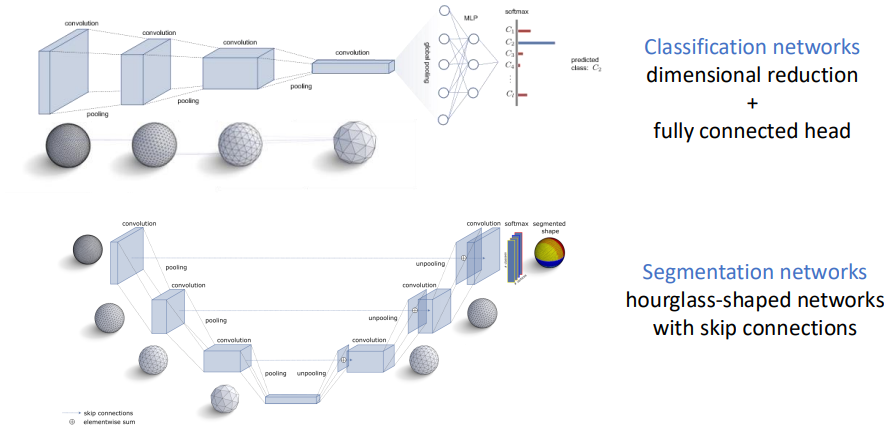
\includegraphics[width=0.7\linewidth]{imgs/lecture19/19.1 network architectures.png}
    \caption{Network architectures}
    \label{fig:19.1}
\end{figure}

\subsubsection{PointNet}
PointNet is the foundational architecture for processing point clouds. It achieves invariance to the order of points through a global pooling operation, which is asymmetric (the result is the same regardless of input order). It uses a learned affine transform to map the point cloud into a common space. And PontNet++, its newer version, adds hierarchical sampling and grouping to better capture local structures within the cloud. 

\subsubsection{Graph-based learning}
Because point clouds are unordered, researchers often impose a graph structure on them to define neighborhoods, like K-nn, where neighbors are defined by spatial proximity or by the similarity of their feature vectors in a higher-dimensional space; or a dynamic graph CNN, which allows the graph neighborhood to update dynamically as the network learns.

\subsubsection{MeshCNN}
MeshCNN is the reference backbone for processing triangle meshes. Unlike point clouds, meshes have explicit connectivity, allowing for specialized convolution operations: edge convolution (the network performs operations directly on the edges of the mesh) and other convolution types (depending on the architecture, convolution can also be centered on half-edges, vertices, or faces).

\section{3D transformers}
Transformers were initially designed to handle sequences of words, but researchers discovered that almost any data, including images, audio, and 3D representations, can be \textbf{tokenized} and interpreted as a sequence. They are particularly useful because they can store foundational knowledge from a massive amount of unlabeled data during pre-training, which can then be applied to specific downstream tasks like 3D editing or completion. \par
There are several critical components that make these networks effective for 3D data:
\begin{itemize}[noitemsep]
    \item \textbf{Tokenization and embedding}: input data is broken down into discrete "tokens", which are then mapped into high-dimensional embedding vectors.
    \item \textbf{Position encoding}: because a transformer processes all tokens simultaneously, it needs a way to distinguish the order of elements in a sequence. This is done by adding frequency-based signals
    \item \textbf{Attention mechanism}: the brain of the transformer. It calculates the mutual importance between tokens, regardless of the initial data type, using query, key, and value metrics. This allows the network to focus on the most relevant parts of a 3D shape during generation.
\end{itemize}

\subsubsection{Output generation}
A major hurdle in 3D generation is that while input embeddings are continuous vectors, the output must be chosen from a finite set, creating an asymmetry between input and output. To solve this, the system uses quantization, meaning that the output space can be a codebook (a dictionary of admissible values or base surface patches). \par
The output token sequence generation strategy uses temperature-based probability space sampling when the network predicts the probability of the next token. If the temperature is zero, it privileges high probability tokens; if the temperature is towards infinity, the random, uniform sampling in the codebook is used.

\subsubsection{Specialized 3D architecture}
There are two landmark models that apply the concepts:
\begin{itemize}[noitemsep]
    \item Point-BERT Encoder: an architecture for point clouds that uses "masked point modeling". It learns by hiding parts of a point cloud and trying to reconstruct them, effectively learning the "grammar" of 3D shapes
    \item Mesh-GPT Decoder: a decoder-only model specifically for triangle meshes. It treats a mesh as a sequence of faces, where each face is a stack of tokens associated with a specialized codebook.
\end{itemize}

\section{3D diffusion models}
These models move away from the direct sequence prediction of transformers to a process based on physics-inspired noise reduction. The core idea behind diffusion is learning to reconstruct data from pure noise:
\begin{itemize}[noitemsep]
    \item Forward diffusion (Training): the system takes a clean 3D object and gradually adds Gaussian noise over many time-steps until the object becomes unrecognizable. The AI learns to predict exactly how much noise was added at each specific step
    \item Reverse diffusion (Inference): to generate a new object, the process is reversed. The system starts with a block of pure Gaussian noise and iteratively removes it, step by step, until a clean 3D shape emerges. This denoising is typically performed by a U-Net architecture.
\end{itemize}

While earlier models like GANs (Generative Adversarial Networks) could produce sharp images, they were often unstable and prone to mode collapse. Diffusion models provide a more stable training objective and a structured latent space, allowing for high-quality, realistic, and diverse 3D generation that was previously difficult to achieve.

\subsubsection{Point-E}
Ponit-E is a diffusion application for point clouds. It uses a fine-tuned model to create a synthetic 2D view from a text prompt and then uses a diffusion model to generate a 3D RGB point cloud based on that image. It can generate complex objects from a prompt.

\subsubsection{PolyDiffusion}
PolyDiffusion is a diffusion solution for meshes. Mesh generation through diffusion is significantly harder because of the need for topological consistency.\par
Instead of a connected mesh, it works on a "triangle soup", where the coordinates of every triangle vertex are quantized. It uses a transformer-based denoiser to iteratively refine the positions of these triangles until they form a coherent 3D polygonal mesh.
